\chapter{Prototipo}
Andiamo ora a mettere in pratica tutto quello che è stato detto su WASI sviluppando un semplice prototipo di una
chat\footnote{\url{https://github.com/ilcors-dev/bachelor-thesis/tree/main/poc}} sviluppata secondo l'architettura a
microservizi.

\section{Architettura}
Il prototipo può essere scomposto in tre layer distinti.

\begin{itemize}
    \item Backend: rappresenta il cuore del prototipo, ed è strutturato secondo un'architettura a microservizi. Ogni
    microservizio è una REST API, è rappresentato da un modulo Wasm e si occupa di una funzionalità specifica
    dell'applicazione
    \item Frontend: rappresenta l'interfaccia grafica resa disponibile agli utenti. Si noti che non è strettamente
    necessaria in quanto grazie all'utilizzo della metodologia REST API è possibile interagire con l'applicazione
    tramite terminale o qualsiasi altro strumento che supporti le richieste HTTP.
    \item Persistenza: rappresenta il layer che gestisce e salva i dati dell'applicazione.
\end{itemize}

\subsection{Le funzionalità}
Le funzionalità dell'applicazione, implementate dal layer backend, sono le seguenti:
\begin{itemize}
    \item Gestione delle chat: si occupa della gestione delle diverse chat presenti, permette la creazione e
    l'eliminazione di esse e può applicare rate limiting ai messaggi.
    \item Gestione dei messaggi: si occupa delle operazioni CRUD (create, read, update, delete) dei messaggi nelle chat
    oltre che della loro sincronizzazione in realtime per i clienti.
    \item Gestione delle sessioni: si occupa della gestione delle sessioni utente, ovvero gli identificativi di ogni
    cliente connesso. È estremamente importante in quanto ogni entità nell'applicazione è legata si lega ad essa.
    \item Gestione degli utenti connessi: è un servizio a fini statistici, in quanto raccoglie il numero degli utenti
    attualmente online e ne permette la lettura.
    \item Gestione del frontend: si occupa della fruizione dell'interfaccia grafica ai clienti dell'applicazione. Può
    essere visto come il filesystem dell'applicazione.
\end{itemize}

\subsection{Le tecnologie backend}
\subsubsection{Rust}
Rust è stato scelto in quanto linguaggio altamente performante e maturo nell'ambiente WebAssembly. È altamente
efficiente grazie alla sua natura di basso livello, alla forte tipizzazione e al sistema di gestione della memoria
altamente ottimizzato. La forte tipizzazione garantisce una bassa probabilità di errori a runtime se comparato ad altri
linguaggi di più alto livello. Si noti che avremmo potuto scegliere qualsiasi altro linguaggio che supporta WebAssembly
per le ragioni di portabilità introdotte in precedenza.

\subsubsection{Wasmtime}
È il runtime utilizzato per eseguire i moduli Wasm e rappresenta il cuore dell'applicazione. Lo abbiamo
\hyperref[sec:capability-example]{già menzionato} quando si è parlato della sicurezza con WASI. È stato scelto per via
della sua conformità allo standard che lo rende una scelta affidabile e robusta per l'esecuzione dei nostri
microservizi.

\subsubsection{Spin Framework}
È un framework basato su Wasmtime che integra in esso le basilari funzionalità necessarie agli scopi del prototipo come
l'interazione con le richieste HTTP, il conseguente routing e la gestione della comunicazione con i database. È uno dei
primi framework presenti nel panorama WASI e per questo motivo è stato scelto per facilitare la realizzazione del
prototipo. Oltre a Rust supporta C/C++, Javascript, Python e Go. Abbiamo in precedenza visto che WASI non espone ancora
in modo stabile alcuna API per il layer networking\footnote{\url{https://github.com/WebAssembly/wasi-sockets}}, per
questo motivo il framework utilizza un'implementazione custom per inizializzare un demone in ascolto per le richieste
HTTP. Questo demone è gestito da WAGI (WebAssembly Gateway Interface)\footnote{\url{https://github.com/deislabs/wagi}}
un'implementazione delle interfacce CGI\cite{RFC3875} per WebAssembly, in grado anche di gestire le richieste in
modalità multi-threaded. Si noti che se anche fosse possibile utilizzare le API standard di WASI per creare il demone,
non lo si potrebbe creare multi-threaded, in quanto anche tale API è ancora in fase di
discussione\footnote{\url{https://github.com/WebAssembly/wasi-threads}}.

\subsubsection{WAGI}
Prima di introdurre WAGI, è utile capire cosa sono le interfacce CGI. Le CGI sono una specifica che permette ai web
server di eseguire programmi a riga di comando ovvero programmi non inizialmente pensati per essere eseguiti in un
ambiente web, e di restituire il risultato al client.

WAGI implementa questa specifica per WebAssembly, esponendo un web
server\footnote{\url{https://github.com/deislabs/wagi/blob/main/src/wagi_server.rs}} HTTP in grado di caricare
dinamicamente i moduli Wasm attraverso
Wasmtime\footnote{\url{https://github.com/deislabs/wagi/blob/main/src/wasm_runner.rs}}. Esegue i moduli mappando i
componenti delle richieste nel seguente modo:
\begin{itemize}
    \item Header = variabili d'ambiente
    \item I parametri della query = argomenti del programma
    \item Il payload = standard input del programma
\end{itemize}

La conseguente risposta dei moduli Wasm viene, come per le CGI, scritta sullo standard output e inviata ai client.

Il valore aggiunto di WAGI è che risulta a sua volta un modulo Wasm eseguito da Wasmtime e è che seppur utilizzi
un'implementazione custom per la gestione delle richieste HTTP e dei thread, segue comunque lo standard WASI in quanto:
\begin{itemize}
    \item Non può accedere ai file del sistema host senza la specifica autorizzazione (capability)
    \item Non può accedere alle variabili del sistema host se non quelle esplicitate da esso
\end{itemize}
ed inoltre
\begin{itemize}
    \item Non può effettuare connessioni di rete esterne
    \item Non può eseguire altre applicazioni che non siano moduli Wasm
\end{itemize}

I moduli Wasm caricati da WAGI vengono chiamati WAGIs ed essendo caricati dinamicamente da Wasmtime non sono processi
esterni, ma sono parte della stessa sandbox. I WAGIs vengono pre-caricati di default e mantenuti in memoria per tutta la
durata dell'esecuzione dell'applicazione.

\subsubsection{Mysql e Redis}
Mysql è un database relazionale che si occuperà di salvare in modo persistente le chat e i messaggi. Redis il secondo è
un datastore che mantiene in memoria dati utili all'applicazione: nel nostro caso il numero di utenti online e le
sessioni attive.

\subsubsection{Docker}
Docker viene utilizzato per la creazione e gestione dei container che ospitano il livello della persistenza dei dati.

\subsection{Le tecnologie frontend}
Non entreremo nel dettaglio delle tecnologie frontend in quanto al di fuori dello scopo della tesi, ma possiamo fornire
una breve descrizione per comprenderle meglio.

\begin{itemize}
    \item ReactJS\footnote{\url{https://github.com/facebook/react}}: un framework Javascript ampiamente utilizzato che consente di creare applicazioni web interattive e
    dinamiche tramite l'uso di componenti - unità di codice riutilizzabili che possono essere combinati per creare
    interfacce grafiche complesse.
    \item TanStackQuery\footnote{\url{https://github.com/TanStack/query}}: una libreria Javascript che facilita la gestione dello stato dell'applicazione e delle chiamate asincrone ai microservizi.
    \item Typescript\footnote{\url{https://github.com/microsoft/TypeScript}}: un linguaggio di programmazione che estende Javascript aggiungendo la tipizzazione statica. Ciò
    permette di scrivere codice più pulito e di prevenire errori di runtime.
    \item Vite\footnote{\url{https://github.com/vitejs/vite}}: uno strumento per lo sviluppo locale e il bundling dei file Javascript e CSS, che permette di
    ottimizzare il carico delle risorse e ridurre i tempi di caricamento delle pagine web.
\end{itemize}

\begin{figure}[h]
    \centering
    \captionsetup{justification=centering}
    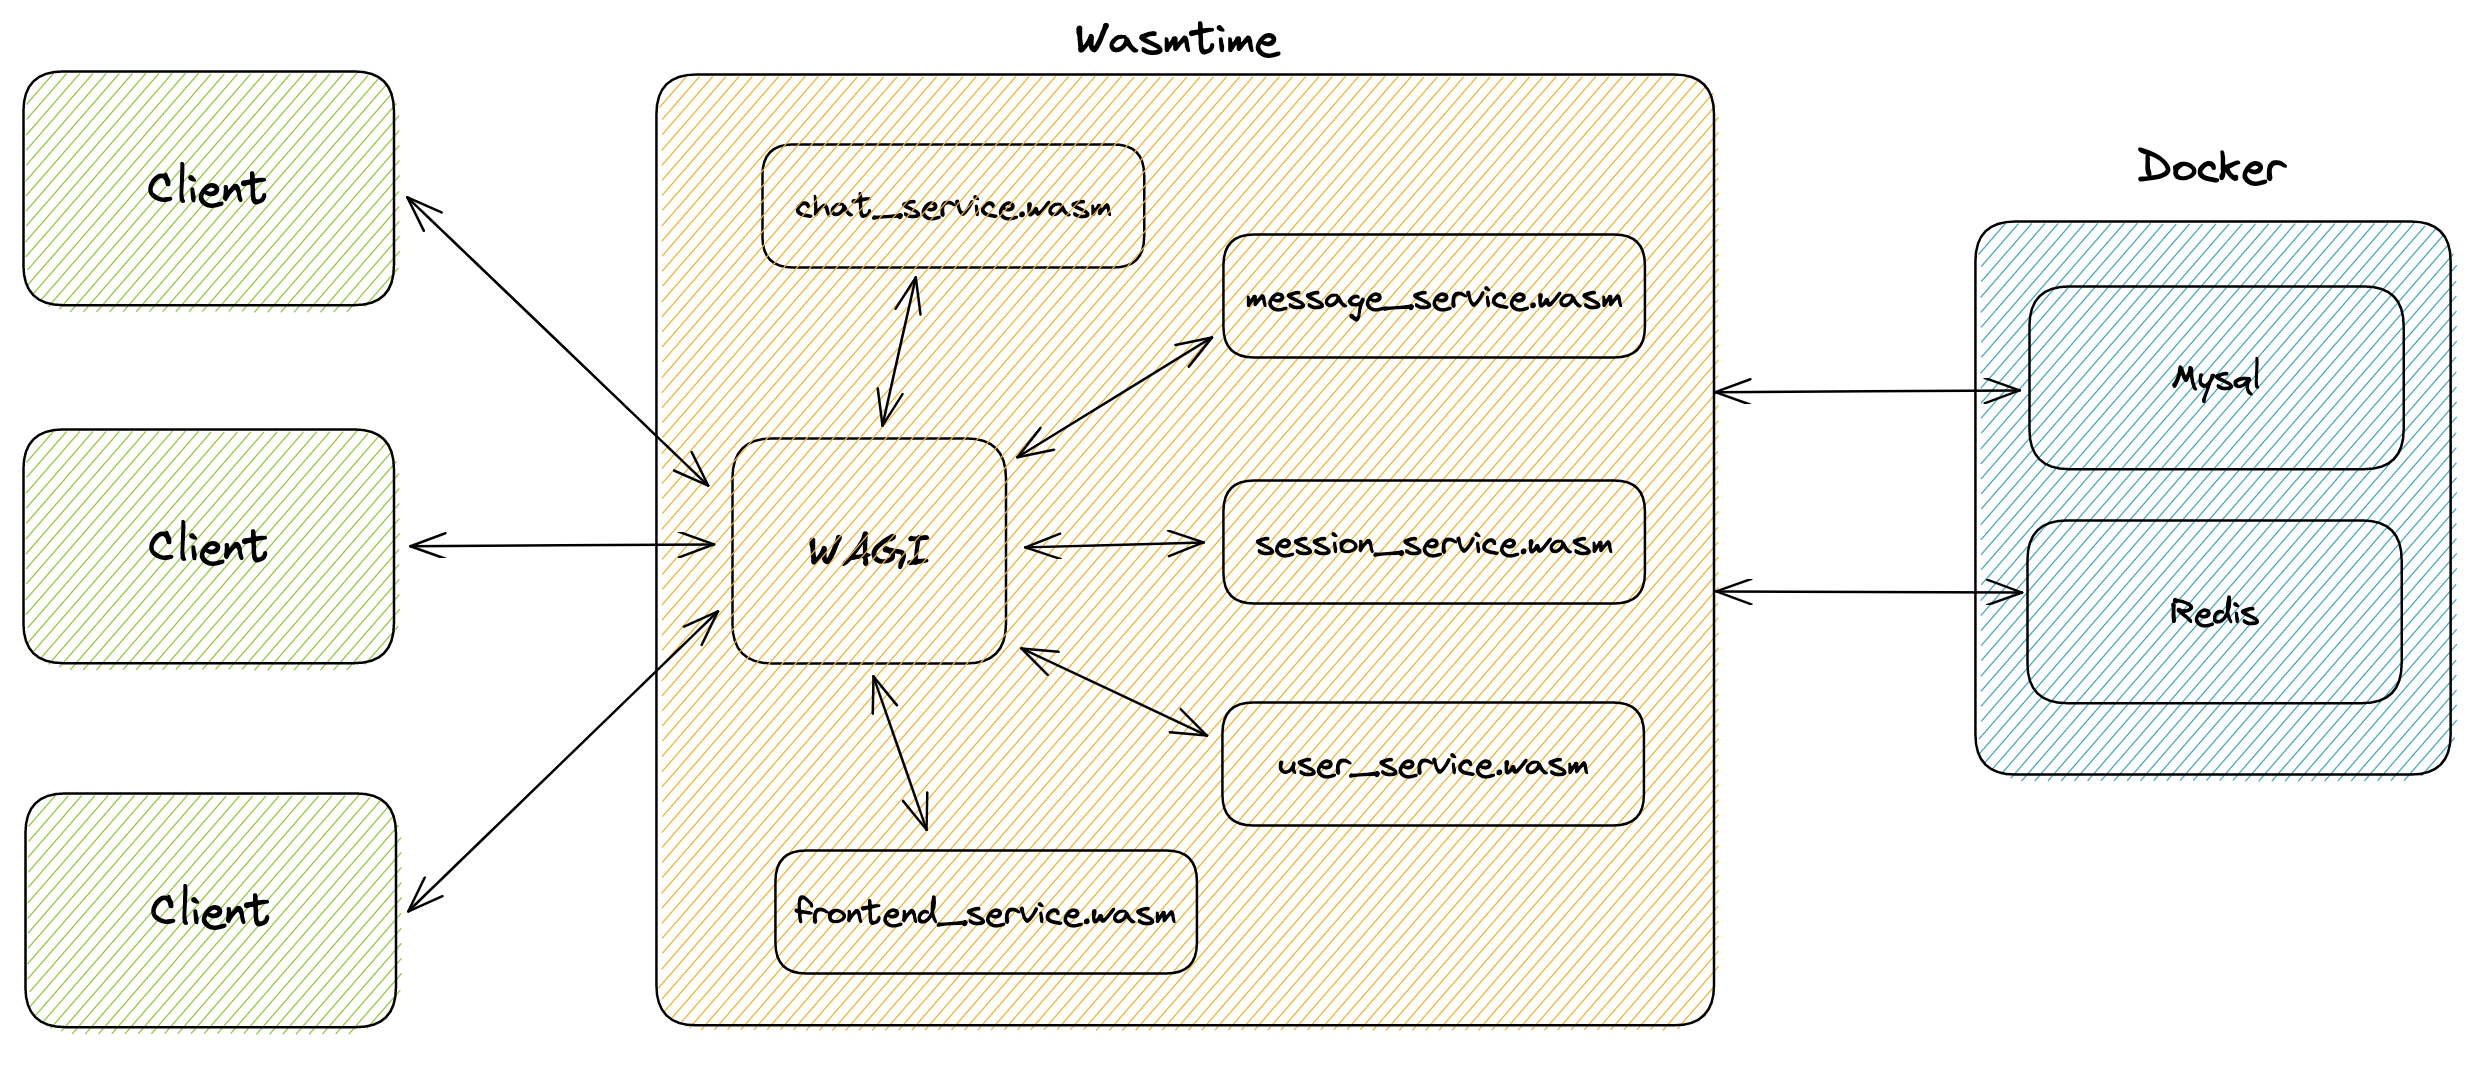
\includegraphics[width=15cm]{./chapters/3.poc/images/0.poc-architecture.png}
    \label{fig:0.poc-architecture}
    \caption{Architettura dell'applicazione}
\end{figure}

\subsection{La configurazione}
La configurazione dell'applicazione avviene modificando il file spin.toml, qui sono presenti varie direttive come la
configurazione delle variabili d'ambiente, del database, di redis e del webserver sottostante. Inoltre qui si
configurano i microservizi presenti nell'applicazione impostando il loro path nella gerarchia delle cartelle, il comando
per eseguire il build e l'url corrispondente ad ognuno di essi. È interessante notare che questo step di mapping tra
url-microservizio-path è necessario poiché il runtime non potrebbe accedere ai vari moduli senza avere le capabilities
necessarie.

\begin{figure}[h]
    \centering
    \captionsetup{justification=centering}
    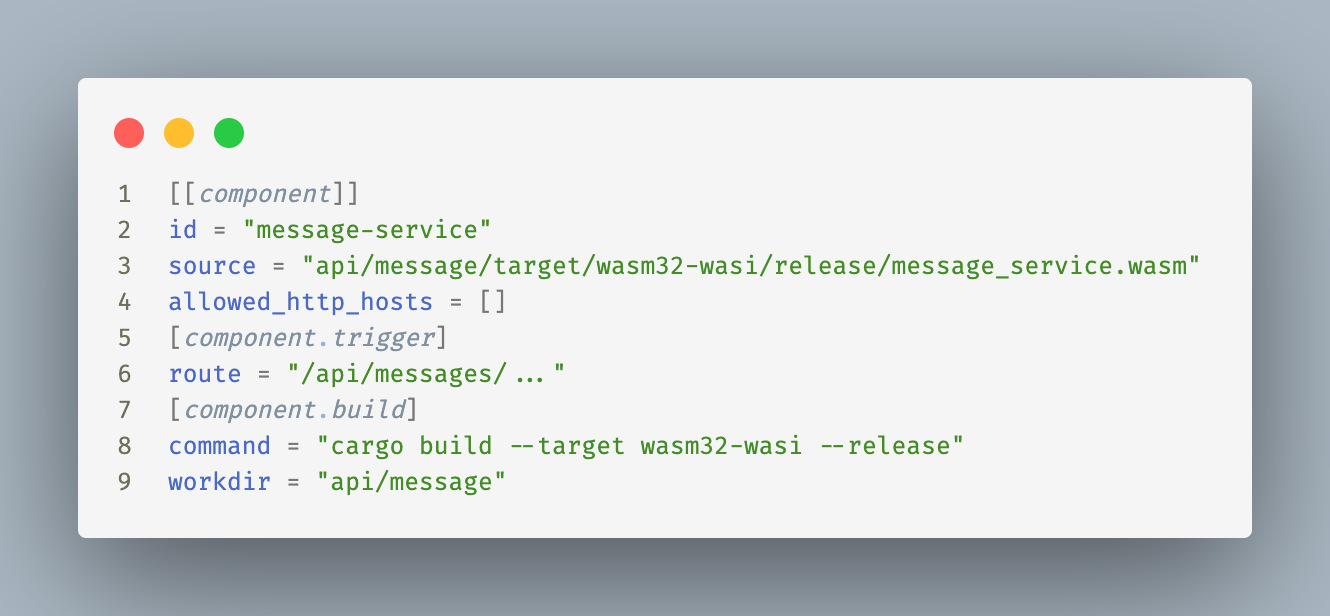
\includegraphics[width=15cm]{./chapters/3.poc/images/1.spintoml.png}
    \label{fig:1.app-configuration}
    \caption{Configurazione di un microservizio}
\end{figure}

Si noti la flag --release nel comando di build, questo è una flag per il compilatore Rust che indica di ottimizzare il
codice durante la compilazione.

\subsection{Interazione}
Parliamo ora di come avviene l'interazione tra le componenti dell'applicazione.

L'applicazione viene avviata tramite il comando spin build --up che esegue il build delle componenti definite in
spin.toml e avvia il web server WAGI in ascolto sulla porta 3000. All'arrivo di una richiesta WAGI richiama il
componente corrispondente all'url richiesto, se lo trova, e lo carica nella sandbox avviandolo con i parametri della
richiesta. Il componente esegue la sua logica e restituisce una risposta al client.

La prima interazione tra client e server è necessaria per generare il token di sessione che identifica il cliente che
verrà usato per tutte le richieste successive. Il token viene generato dal session\_service e viene salvato sul
database. Una volta ricevuto il token il cliente potrà effettuare richieste al server.

% Un utente può essenzialmente fare due cose: interagire con le chat e scrivere messaggi. Ogni 

\subsubsection{Una nota sulla sincronizzazione realtime}
La sincronizzazione dei dati in tempo reale tra client e server è effettuata tramite un'interazione a polling. Il motivo
di questa scelta è dato dal fatto che al momento della scrittura del documento WASI non supporta la gestione delle
WebSocket.

\section{Un confronto con le soluzioni esistenti}

\subsection{Benchmark}

\subsection{Il deployment}
\section{Vantaggi e Svantaggi}


\section{Conclusione}